\documentclass[aps,superscriptaddress]{revtex4}

\textheight      9.9in
\textwidth       6.7in
\topmargin      -0.5in

%your favourite packages here
\usepackage[spanish]{babel}
% \usepackage{lineno}
% \usepackage{mathptmx}
\usepackage{sublabel}
%\usepackage{psfrag,graphicx}
\usepackage{subfigure} 
\usepackage{amsmath} 
\usepackage{amssymb} 
\usepackage{amsfonts}
\usepackage{bm}
%\usepackage{bbm}
\usepackage{color}
\usepackage{overpic}
\usepackage{latexsym}
\usepackage{epstopdf}
\usepackage{color}
%\usepackage{times}
\usepackage{stmaryrd}

\usepackage{psfrag,graphicx} 
%\usepackage{picins} 
\usepackage{epsf} 
\usepackage{natbib}
\usepackage{epstopdf}\DeclareGraphicsRule{.tif}{png}{.png}{`convert #1 `basename
#1 .tif`.png}
\usepackage{appendix}
%\usepackage{dsfont}
%\usepackage{mathtools}

\definecolor{mygrey}{gray}{0.35}
\definecolor{myblue}{rgb}{0.2,0.2,0.8}
\definecolor{myzard}{cmyk}{0,0,0.05,0}
\definecolor{mywhite}{rgb}{1,1,1}
\definecolor{myred}{rgb}{1,0.,0.3}

%\definecolor{myblue}{named}{MidnightBlue}
\usepackage[colorlinks=true,citecolor=myblue,linkcolor=myred]{hyperref}
\def\beq{\begin{equation}}
\def\eeq{\end{equation}}
\def\ba{\begin{align}}
\def\enda{\end{align}}
\def\bi{\begin{itemize}}
\def\ei{\end{itemize}}
\def\bs#1{\boldsymbol{#1}}
\def\txt#1{\textrm{#1}}

\newcommand{\eq}[1]{Eq.\;(\ref{#1})}

\newcommand{\sgn}{\operatorname{sgn}}
\def\C{{\mathbb{C}}} \def\F{{\mathbb{F}}}
\def\N{{\mathbb{N}}} \def\Q{{\mathbb{Q}}}
\def\R{{\mathbb{R}}} \def\Z{{\mathbb{Z}}}
\def\cH{{\mathcal H}}
\def\bfsigma{\boldsymbol{\sigma}}
\def\bfmu{\boldsymbol{\mu}}
\def\dd{\mathord{\rm d}} \def\Det{\mathop{\rm Det}}
\def\dist{\mathop{\rm dist}} \def\ee{\mathord{\rm e}}
\def\End{\mathord{\rm End}} \def\ev{\mathord{\rm ev}}
\def\id{\mathord{\rm id}} \def\ii{\mathord{\rm i}}
\def\min{\mathord{\rm min}} \def\mod{\mathord{\rm mod}}
\def\prob{\mathord{\rm prob}}
\def\tr{\mathop{\rm Tr}}
\def\half{\textstyle\frac{1}{2}}
\def\third{\textstyle\frac{1}{3}}
\def\fourth{\textstyle\frac{1}{4}}

\graphicspath{{figs/}}

\newcommand{\da}{\downarrow}
\newcommand{\ua}{\uparrow}

\renewcommand{\ii}{{\rm i}}
\renewcommand{\ee}{{\rm e}}

%brackets
 \newcommand{\ket}[1]{|#1\rangle}
 \newcommand{\bra}[1]{\langle #1|}
 \newcommand{\braket}[2]{\langle #1|#2\rangle}

 \newcommand{\ketbra}[2]{\ket{#1}\bra{#2}}
 \newcommand{\proj}[1]{\ketbra {#1}{#1}}
 \newcommand{\biket}[2]{\ket{#1\;#2}}
 \newcommand{\bibra}[2]{\bra{#1\;#2}}
 %\newcommand{\ketbradif}[2]{\biket {#1}{#2}\bibra {#1}{#2}}
 \newcommand{\preespacio}{\!\text{\hspace{0.2 ex}}}
 \newcommand{\postespacio}{\!\text{\hspace{0.75 ex}}}


% \graphicspath{{Plots/}}

\begin{document}

%\title[Short Title]{Ejercicios para el curso de Introducci\'on a la \'Optica Cu\'antica}

\author{C. Cormick}

% \maketitle

\noindent{\large \bf Procesamiento Cu\'antico de la Informaci\'on - C. Cormick, FING - 1er sem. 2025}\\

\noindent{\large \bf Práctico 1 - Qubits, estados cuánticos, compuertas y mediciones}\\

\vspace{20pt}

\noindent Aclaraci\'on: Estos ejercicios fueron tomados de o inspirados en ``Virginia Tech Quantum Information Science and Engineering Summer School 2022'' por Sophia E. Economou, Edwin Barnes, y Jamie Sikora. A su vez su enfoque y notaci\'on son en buena medida de ``Q is for Quantum'', de Terry Rudolph.

\medskip

\begin{enumerate}
\item {\bf Compuertas cl\'asicas y notaci\'on gr\'afica.} Hallar los colores de salida de los bits en el siguiente circuito (recordar que el blanco representa 0 y el negro 1):

\begin{center}
 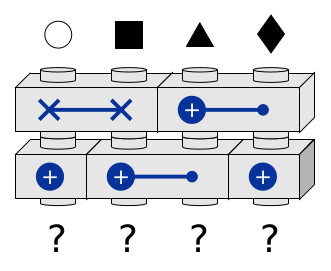
\includegraphics[width=110pt]{compuertas_clasicas_1.png}
\end{center}

\item {\bf Desaf\'ios:}

\begin{enumerate}
    \item Hallar cuatro circuitos diferentes que contengan como mucho dos compuertas cl\'asicas y que den origen a la regla de entrada-salida graficada a continuaci\'on:

    \begin{center}
    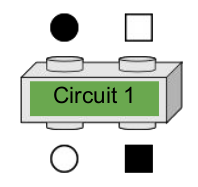
\includegraphics[width=70pt]{problema2_a.png}
    \end{center}

    \item De esos cuatro circuitos, cu\'ales respetan las siguientes reglas de entrada-salida?
    
    \begin{center}
    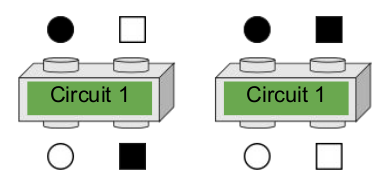
\includegraphics[width=145pt]{problema2_b.png}
    \end{center}
    
    \item Y cu\'ales las que siguen?
    
    \begin{center}
    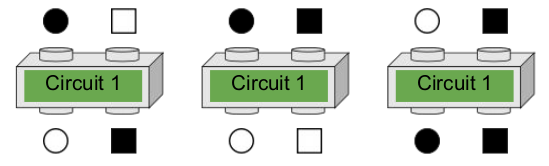
\includegraphics[width=220pt]{problema2_c.png}
    \end{center}
    
    
    \item Y ahora?
    
    \begin{center}
    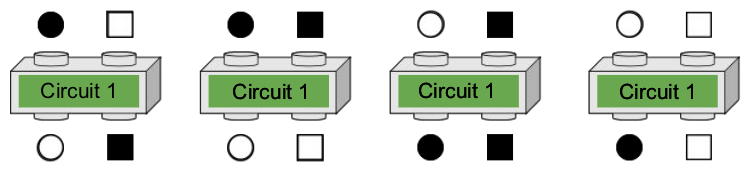
\includegraphics[width=290pt]{problema2_d.png}
    \end{center}

\end{enumerate}


    \newpage
    
    \item {\bf Estados ``neblinosos'' y mediciones:} Indicar cu\'ales son los posibles resultados al medir en el siguiente circuito (la salida deben ser dos bits!). Dibujar el estado final correspondiente en cada caso.

    \begin{center}
    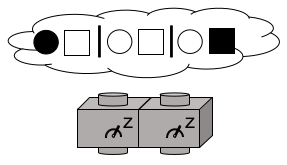
\includegraphics[width=115pt]{medicion1.png}
    \end{center}

    
\item {\bf Estados ``neblinosos'' y compuertas cu\'anticas:} 

    \begin{enumerate}
    \item Dise\~nar un posible circuito en el que, ingresando dos qubits en cero, la salida sea el estado:
    
    \begin{center}
    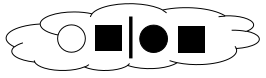
\includegraphics[width=100pt]{neblinoso_1.png}
    \end{center}

    \item Hallar el estado de salida para el siguiente circuito:

    \begin{center}
    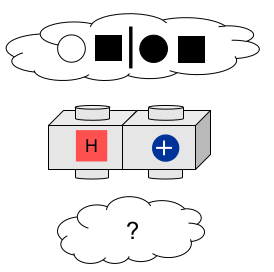
\includegraphics[width=105pt]{neblinoso_2.png}
    \end{center}

    \item Indicar los posibles resultados si se miden los dos bits a la vez.
    
    \end{enumerate}
    
    \smallskip

    \item {\bf Manipulaci\'on de estados neblinosos (o en ``superposici\'on cu\'antica'')}
    
    \begin{enumerate}
        \item Reescribir los siguientes estados neblinosos de la forma m\'as simple posible:
    
        \begin{center}
        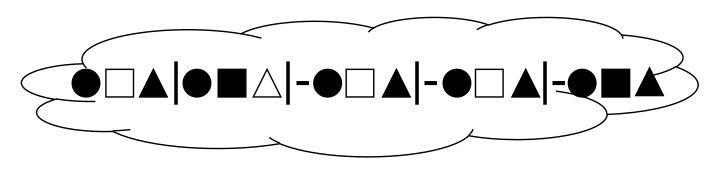
\includegraphics[width=250pt]{simplify1.png}\vspace{5pt}\\
        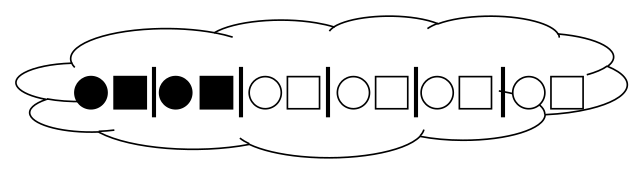
\includegraphics[width=190pt]{simplify2.png}
        \end{center}
    
        \item Distribuir el siguiente estado de tres qubits de modo que quede todo dentro de una \'unica ``neblina'':
    
        \begin{center}
        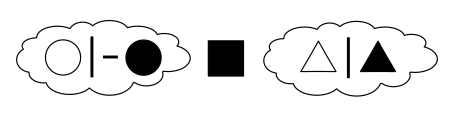
\includegraphics[width=130pt]{combine_mist.png}
        \end{center}
        
        \newpage
    
        \item Factorizar los siguientes estados neblinosos lo m\'as posible en t\'erminos de estados de los diferentes qubits:    
        \begin{center}
        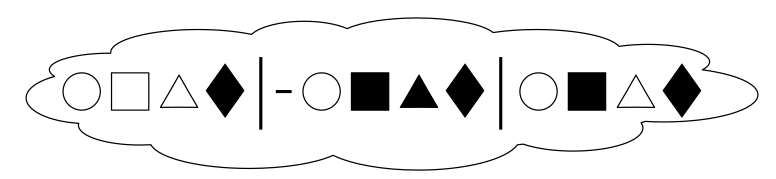
\includegraphics[width=200pt]{factor_mist_1.png}\vspace{5pt}\\
        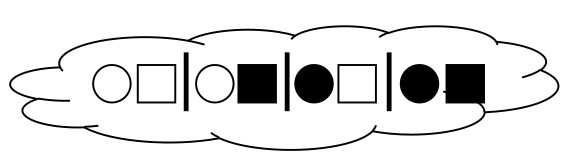
\includegraphics[width=140pt]{factor_mist_2.png}\vspace{5pt}\\
        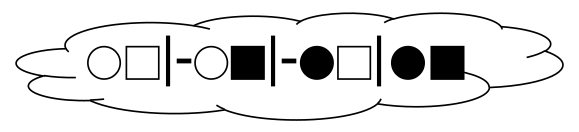
\includegraphics[width=170pt]{factor_mist_3.png}
        \end{center}

    \end{enumerate}

    \item {\bf Circuitos cu\'anticos.} Consideramos los siguientes circuitos:\vspace{-10pt}\\
    \begin{center}
    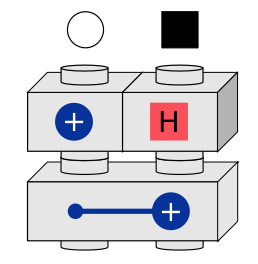
\includegraphics[width=75pt]{simple_circuit_1.png}\hspace{30pt}
    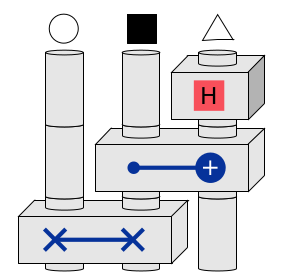
\includegraphics[width=100pt]{simple_circuit_2.png}
    \end{center}
    
    \begin{enumerate}
     \item Indicar el estado de salida en cada caso.
     \item Indicar si el estado de salida se puede factorizar en estados de cada qubit.
     \item Si al final del circuito se miden todos los qubits, explicar cu\'ales son los posibles resultados y sus correspondientes probabilidades.
    \end{enumerate}

    \item {\bf Mediciones completas y parciales:}
    
    \begin{enumerate}
        \item Volver a considerar el problema 3. Indicar cu\'al es la probabilidad de hallar cada uno de los resultados posibles.
    
        \item Suponer ahora que en vez de medir ambos qubits solo se mide el segundo, lo cual gr\'aficamente se representa as\'i:
        
        \begin{center}
        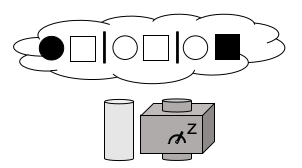
\includegraphics[width=125pt]{partial_measurement.png}
        \end{center}
        
        Indicar ahora cu\'ales son los posibles resultados al medir ese \'unico qubit, y cu\'ales son las respectivas probabilidades.
        
        \item Suponiendo la medici\'on del \'item anterior, indicar cu\'al es el estado luego de la medici\'on de acuerdo al resultado obtenido.
        
    \end{enumerate}

    \item {\bf Mediciones y colapso.} Volver a considerar el primer estado del problema 5.c, de 4 qubits.
    
    \begin{enumerate}
     \item Supongamos que medimos el qubit representado por un cuadrado y vemos que es negro. Dibujar el estado de los 4 qubits despu\'es de la medici\'on.
     \item Ahora volvamos a considerar el mismo estado inicial, pero en vez de medir el qubit cuadrado medimos el tri\'angulo, y obtenemos negro. Nuevamente dibujar el estado de los 4 qubits despu\'es de la medici\'on.
     \item Otra vez suponiendo el mismo estado inicial, digamos que medimos el qubit tri\'angulo y el rombo, y obtenemos blanco y negro respectivamente. Dibujar el estado final correspondiente.
    \end{enumerate}

    \newpage
    
    \item {\bf Adivinar circuitos.} Sabemos que un circuito tiene el comportamiento de la figura:
    
        \begin{center}
        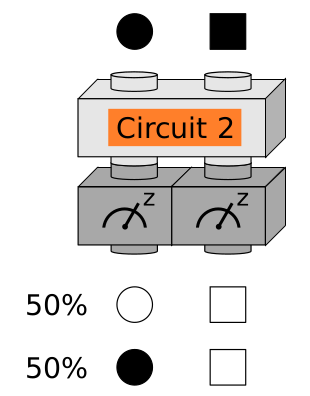
\includegraphics[width=90pt]{circuit_finding.png}
        \end{center}
    
    Es decir, si el input son dos qubits negros, al medir ambos qubits luego de pasar por el circuito, con 50\% de probabilidad se mide ``blanco-blanco'' y con 50\% ``negro-blanco''.
    
    \begin{enumerate}
     \item Cu\'al es la probabilidad (para ese mismo estado de entrada) de que al medir el qubit cuadrado el resultado sea blanco?
     \item Encontrar dos circuitos de como m\'aximo dos compuertas y que respeten estas reglas de entrada-salida.
     \item Optativo: para esos circuitos hallados en el \'item anterior, es posible encontrar un estado neblinoso de entrada que al pasar por el circuito se vuelta un estado cl\'asico (o sea, sin neblina)?
    \end{enumerate}

%    \item {\bf Compuerta Z.} Mostrar que aplicar sobre un qubit la compuerta Z seguida de la X da lo mismo que aplicar primero la X y luego la Z.
    
    \item {\bf Compuerta C-Z.} Calcular las reglas de entrada-salida para los circuitos de las figuras. A qu\'e compuerta conocida son equivalentes estas combinaciones?
    
    \begin{center}
     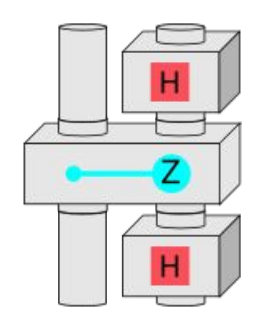
\includegraphics[width=75pt]{CZ1.png}
     \hspace{40pt}
     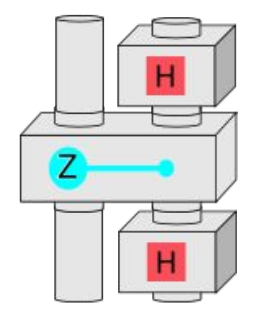
\includegraphics[width=75pt]{CZ2.png}
    \end{center}

    \item {\bf Toffoli.} La compuerta de Toffoli es una compuerta cl\'asica de tres bits con las reglas de entrada-salida que se muestran en la figura, es decir, que cambia el valor del bit ``target'' si y solo si ambos bits de control valen 1 (en nuestro caso, son negros).
    
    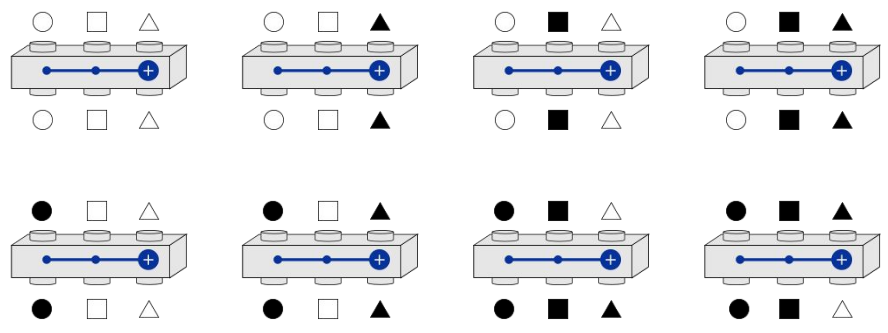
\includegraphics[width=460pt]{Toffoli_reglas.png}

    \begin{enumerate}
     \item Explicar c\'omo se puede usar compuertas de Toffoli para implementar compuertas CNOT.
     \item Qu\'e pasa si se aplican dos compuertas de Toffoli consecutivas sobre los mismos bits (con los mismos controles y target)?
     \newpage
     \item Ahora consideramos que en vez de bits tenemos qubits. Hallar las reglas de entrada-salida para el circuito de la figura:
    \end{enumerate}

    \begin{center}
     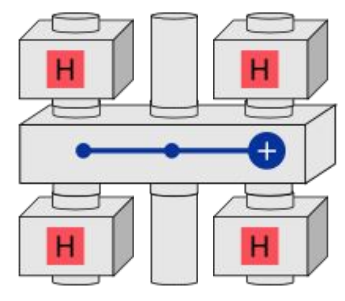
\includegraphics[width=100pt]{Toffoli_H.png}
    \end{center}
    
    \end{enumerate}

\vspace{20pt}

    
    \noindent{\large \bf Parte 2 - IBM Quantum Experience}

\vspace{20pt}

Entrar a IBM Quantum Composer (\href{https://quantum.ibm.com/composer}{https://quantum.ibm.com/composer}). Es posible abrir una cuenta personal (esto es lo mejor para salvar archivos y continuar trabajando sobre ellos en otra sesi\'on), pero tambi\'en se puede comenzar a usar el simulador sin tener ninguna cuenta. \\

Los paneles ``Q-sphere'' y ``Statevector'' no vamos a usarlos y lo mejor es cerrarlos. En cambio, s\'i queremos ver los paneles ``Graphical editor'' y ``Probabilities''. El panel de la derecha es el editor de c\'odigo, complementario del editor gr\'afico y lo pueden cerrar, o usarlo si les resulta c\'omodo y/o quieren ir aprendiendo a escribir c\'odigo (hay a su vez dos opciones para escribir, ``QASM'' y ``Qiskit'', pueden explorar ambas y ver cuál les resulta mejor).\\

Dentro del editor gr\'afico, tenemos l\'ineas grises horizontales que representan los qubits q[j], con j indicando cada qubit, otras l\'ineas grises m\'as abajo que representan bits que guardan los resultados de las mediciones, cajitas que representan compuertas cu\'anticas y otras que representan mediciones. Las cajitas se pueden tomar del men\'u, arrastrar y colocar en la posici\'on deseada.\\

Las l\'ineas que representan el registro cl\'asico tienen a la izquierda un indicador ``cj'' donde j es el n\'umero total de bits cl\'asicos. Tanto los qubits como los bits se numeran con enteros empezando por el cero. Cuando se coloca una medici\'on, las cajitas que representan la medida vienen con una l\'inea punteada que apunta al registro cl\'asico; al lado de esta l\'inea figura el \'indice del bit que guardar\'a el resultado. Este \'indice se puede cambiar en el editor de texto, o haciendo doble clic sobre la cajita de medici\'on.\\

Cada qubit empieza en el estado 0 (blanco); para cambiar esto, se puede agregar una compuerta NOT al empezar. La evoluci\'on de los qubits es de izquierda a derecha; se puede pensar como en el formalismo gr\'afico de los ejercicios pasados, excepto que rotando todo en 90$^\circ$ en sentido antihorario:

\begin{center}
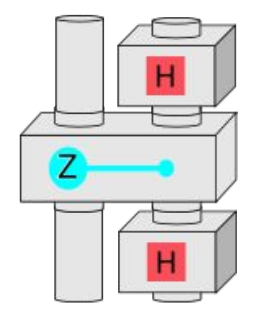
\includegraphics[width=70pt]{CZ2.png}\quad\raisebox{35pt}{$\rightarrow$}\quad\raisebox{5pt}{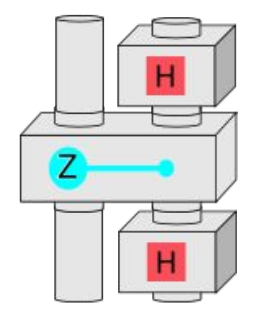
\includegraphics[width=70pt, angle=90]{CZ2.png}}
\end{center}

El panel ``Probabilities'' muestra un diagrama de barras con las probabilidades de los diferentes resultados al realizar una medici\'on. Las probabilidades se calculan a trav\'es de un simulador cl\'asico, pero tambi\'en es posible pedir que el circuito se implemente en un procesador cu\'antico verdadero. En este caso, es imprescindible colocar los s\'imbolos de medici\'on al final del circuito. Notar que si se implementa la simulaci\'on cl\'asica y no se colocan compuertas de medici\'on, el panel ``Probabilities'' indica el resultado de medir todos los qubits y almacenar el resultado del qubit j en el bit j.\\

En el caso de simulaciones cl\'asicas, la aleatoriedad cu\'antica es simulada con n\'umeros pseudoaleatorios. En el caso de utilizar procesadores cu\'anticos, a la aleatoriedad cu\'antica se suma la presencia de ruido, que hace que los resultados sean diferentes de los obtenidos en la simulaci\'on. Si bien en general tiene m\'as sentido usar los simuladores cl\'asicos, cada tanto puede ser un buen ejercicio comparar los resultados con los de un procesador cu\'antico.\\

\newpage

\begin{enumerate}
 \setcounter{enumi}{11}

    \item {\bf Ejercicios para arrancar:}
    
    \begin{enumerate}
        \item Empezar por considerar un solo qubit, y ver qu\'e pasa si se coloca una compuerta NOT ($\oplus$), o dos consecutivas. (El ``quantum composer'' arranca con 4 qubits y 4 bits, pero haciendo clic sobre los qubits se los puede borrar y haciendo clic sobre los bits se puede cambiar su número.)
 
        \item Verificar tambi\'en que los resultados sean razonables si se coloca alguna compuerta Hadamard (H) o dos consecutivas.
 
        \item Agregar otro qubit, y reconocer a qu\'e bit corresponde cada d\'igito en las probabilidades, colocando compuertas NOT en diferentes l\'ineas y viendo c\'omo cambian los resultados. Ver tambi\'en qu\'e pasa si se coloca una compuerta Hadamard sobre uno de los qubits, o sobre los dos.
 
        \item Para un circuito con dos qubits, colocar una compuerta CNOT y ver c\'omo cambian los resultados si los qubits se inicializan en 00, 01, 10, 11 (colocando compuertas NOT al principio donde sean necesarias).
        
        \item Implementar el circuito del problema 1. Verificar que el resultado sea consistente con el obtenido antes.
        
    \end{enumerate}
    
    \item Implementar el circuito de la figura:\vspace{-25pt}\\    
    \begin{center}
     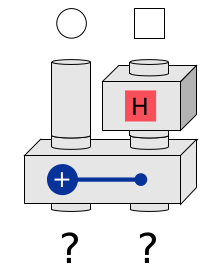
\includegraphics[width=70pt]{guia2_prob2.png}
    \end{center}
    
    \begin{enumerate}
     \item Cu\'ales son los posibles resultados de una medici\'on final sobre los dos qubits?
     \item Para cada resultado, qu\'e propiedades tienen los colores de los dos qubits / valores de los dos bits?
     \item Calcular el estado de salida de los qubits a mano y comparar con los resultados de las mediciones seg\'un el simulador.
%     \item Es posible factorizar el estado de salida de los qubits previo a la medici\'on?
    \end{enumerate}

    \item Implementar los circuitos correspondientes a los problemas 2, 9 y 10. Chequear los resultados.

    \item Implementar el circuito de la siguiente figura:\vspace{-15pt}\\    
    \begin{center}
     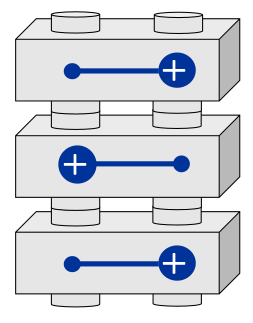
\includegraphics[width=65pt]{concat_CNOTs.png}
    \end{center}
    
    \begin{enumerate}
     \item Probar todos los posibles valores de los bits de entrada y registrar las correspondientes salidas. 
     
     \item C\'omo cambian las reglas de entrada-salida si se agrega una compuerta SWAP al final del circuito?
     
     \item Qu\'e compuerta cl\'asica tiene las mismas reglas de entrada-salida que la concatenaci\'on de la figura? Verificar haciendo la cuenta a mano, notando que se trata solo de compuertas cl\'asicas, y que la acci\'on del CNOT se puede escribir como una suma m\'odulo 2.

    \end{enumerate}
    
    \item Verificar con el simulador IBM las respuestas al problema 11.

\end{enumerate}


\end{document}
